\documentclass [11pt, a4paper, oneside] {article}
\usepackage {amsmath}
\usepackage {geometry}
\geometry{left=2.5cm,right=2.5cm}
\usepackage {amssymb}
\usepackage {graphicx}

\usepackage{multirow}
\linespread{1.5}
\usepackage[procnames]{listings}
\usepackage{color}
\usepackage {pythonhighlight} 
\author {Yue Wang, A53102167}
\title {CSE250A Homework3 Answer}
\begin {document}
\maketitle
\section *{3.1 Inference}
This model is a Markov chain, which means the distribution of each node only depends on the immediate previous node and the transmission probabilities. We can also view this in using conditional independence that every node conditional independent to its previous node except its immediate previous node given its immediate previous node.\\
\subsection *{(a)}
In this question, I will prove it using induction.\\
If t = 1, we have: $P(X_{2}=j|X_1=i) = A^1_{ij}$, which is true from the definition of P.\\
Assume t = n, we have:
$P(X_{n+1}=j|X_1=i) = [A^n]_{ij}$\\
When t = n+1:\\
$P(X_{n+2}=j|X_1=i) = \sum\limits_{k=1}^{m}P(X_{n+2}=j, X_{n+1}=k|X_1=i) = \sum\limits_{k=1}^{m}P(X_{n+2}=j|X_{n+1}=k, X_1=i)P(X_{n+1}=k| X_1=i)
 = \sum\limits_{k=1}^{m}P(X_{n+2}=j|X_{n+1}=k)P(X_{n+1}=k| X_1=i) = \sum\limits_{k=1}^{m}A_{kj}*[A^n]_{ik} = \sum\limits_{k=1}^{m}[A^n]_{ik}*A_{kj} 
 = [A]^{n+1}_{ij} $\\ (According to the definition of matrix production, if $C = A*B, C_{ij} = \sum\limits_{k=1}^{m}A_{ik}B_{kj}$ where m is the number of columns of A and the number of rows of B)\\
\subsection *{(b)}
When we do the inference, one possible way is to use get the $A^t$ first which the complexity is $O(m^3t)$(When doing matrix multiplication, the plain way takes 
$O(m^3)$ and there are totally t matrix multiplications). Then use marginalization to get the $P(X_{t+1}=j)$,  because $P(X_{t+1}=j) = \sum\limits_{i=1}^{m}P(X_{t+1}=j, X_1=i) = 
\sum\limits_{i=1}^{m}P(X_{t+1}=j|X_1=i)P(X_1=i)$. And the time complexity is $O(m^3t+m) = O(m^3t)$\\
However there are more information than we need in $A^t$. So let's analyze our object again and look for a new efficient algorithm. \\
Let's define $V_{X_i} = [p_{X_{i1}}, p_{X_{i2}}, \cdots, p_{X_{im}}]$ as the probability vector which denotes the probability distribution of $X_i$. ($p_{X_{ik}}$ denotes the probability of $X_{i} = k$)\\
Then $V_{X_1}$ is the initial probability distribution of the model.\\
Our objective is to get $V_{X_{t+1}}$, where $V_{X_{t+1}} = V_{X_{t}}*A,$ where $V_{X_{t}} = V_{X_{t-1}}*A, \cdots, V_{X_{2}} = V_{X_{1}}*A$\\
There are totally t vector-matrix multiplications and each vector-matrix multiplication takes $O(m^2)$ steps. So the time complexity is $O(m^2t).$\\
Proof of $V_{X_{i}} = V_{X_{i-1}}*A$:\\
$V_{X_{i}k} =  p_{X_{ik}} = \sum\limits_{j=1}^{m}P(X_{i}=k, X_{i-1}=j) = \sum\limits_{j=1}^{m}P(X_{i}=k|X_{i-1}=j)P(X_{i-1}=j) = \sum\limits_{j=1}^{m}A_{jk}*V_{X_{i-1}j} = 
V_{X_{i-1}}*A_{*k}$ where $A_{*k}$ denotes the kth column of A\\
So $V_{X_{i}} = V_{X_{i-1}}*A$\\
\subsection *{(c)}
We know the complexity of $A*A$ is $O(m^3)$ and if we want to get $A^{t+1}$ step by step, we will do t times matrix production where the time complexity is $O(m^3t)$\\
However, an alternate way is to calculate the matrix production using divide and conquer. We can calculate $A^{t+1}$ in the following way:\\
$A^{t+1} = A^{\frac{t+1}{2}}*A^{\frac{t+1}{2}}, $ if t+1 is even. $A^{t+1} = A^{\frac{t+1}{2}}*A^{\frac{t+1}{2}}*A, $ if t+1 is odd\\
$A^{\frac{t+1}{2}} = A^{\frac{t+1}{4}}*A^{\frac{t+1}{4}}, $ if $\frac{t+1}{2}$ is even. $A^{\frac{t+1}{2}} = A^{\frac{t+1}{4}}*A^{\frac{t+1}{4}}, $ if $\frac{t+1}{2}$ is odd\\
$\cdots$\\
Do this recursively until \\
$A^{2} = A*A$ or $A^{3} = A*A*A$\\
And there are totally $O(\log_2t)$ steps, in each step, it takes $O(m^3)$ to do the matrix production. So the whole work can be done in $O(m^3\log_2t)$\\
\subsection *{(d)}
Since the matrix is extremely sparse, we need to look for a new way to represent the transition matrix. \\
Let's define a new array S whose size is m. And each entry is a list. In the previous matrix, if $A_{ij}$ is non-zero, we add a pair $(j, A_{ij})$ to the S[i]. Totally, there are O(sm)  $(j, A_{ij})$ pairs.\\
If we want to get the distribution of $X_{t+1}$, we can calculate the distribution of $X_1, X_2, X_3, \cdots, X_{t}, X_{t+1}$ step by step, because $X_{t+1}$ only depends on $X_{t}$\\
Assume we have the distribution of $X_{t+1}$, then\\
$P(X_{t+1}=k) = \sum\limits_{i=1}^{m}P(X_{t+1}=k|X_{t}=i)P(X_{t}=i)$\\
So if $P(X_{t+1}=k|X_{t}=i)=0$, there is no need to do the calculation $P(X_{t+1}=k|X_{t}=i)*P(X_{t}=i)$, so we can concentrate on that $P(X_{t+1}=k|X_{t}=i)\neq0$, namely, $A_{ik}\neq0$, which the number of is O(sm)\\
Let's define $V_{X_i} = [p_{X_{i1}}, p_{X_{i2}}, \cdots, p_{X_{im}}]$ as the probability vector which denotes the probability distribution of $X_i$. ($p_{X_{ik}}$ denotes the probability of $X_{i} = k$)\\
In our privious array S, there are totally O(sm) $(k, A_{ik})$ paris. We can loop over these paris and when we see a pair whose the first element is k, we can add $P(X_{t}=i)*A_{ik}$ to $p_{X_{(t+1)m}}$. And after we loop over all the pairs, which takes O(sm) time, we get the distribution of $X_{t+1}$. And from $X_{1}$ to $X_{t+1}$, there are t steps. So the time complexity is O(smt)\\
\section *{3.2 Stochastic simulation}
\subsection *{(a)}
Proof:\\
$\sum\limits_zP(Z=z|B_1, B_2, \cdots, B_n) = \sum\limits_z(\frac{1-\alpha}{1+\alpha})\alpha^{|z-f(B)|}$\\
Because f(B) is a constant number when the n is fixed, $z-f(B)\in [-\infty, +\infty]$ and it is an integer\\
Let $x = z-f(B)$ and $x \in [-\infty, +\infty]$ and x is an integer\\
$\sum\limits_zP(Z=z|B_1, B_2, \cdots, B_n) = \sum\limits_z(\frac{1-\alpha}{1+\alpha})\alpha^{|z-f(B)|} = \sum\limits_x(\frac{1-\alpha}{1+\alpha})\alpha^{|x|} $ where $x \in [-\infty, +\infty]$ and x is an integer\\
$\sum\limits_zP(Z=z|B_1, B_2, \cdots, B_n) = (\frac{1-\alpha}{1+\alpha})(\sum\limits_x(2*\alpha^{x}) - 1) $ where $x \in [0, +\infty]$ and X is an integer(Omitted in the following proof).\\
We can see $\alpha^{x}$ is a geometric progression. So:\\
$\sum\limits_{x=0}^{+\infty}(2*\alpha^{x}) - 1 = 2*\lim\limits_{x\to\infty}\frac{1-\alpha^{x}}{1-\alpha} - 1 = \lim\limits_{x\to\infty}\frac{2-2\alpha^{x}-1+\alpha}{1-\alpha} =
\lim\limits_{x\to\infty}\frac{1-2\alpha^{x}+\alpha}{1-\alpha} = \frac{1+\alpha}{1-\alpha}$\\
$\sum\limits_zP(Z=z|B_1, B_2, \cdots, B_n)  =  (\frac{1-\alpha}{1+\alpha})(\frac{1+\alpha}{1-\alpha}) = 1$ where $z \in [-\infty, +\infty]$ and z is an integer\\
\subsection *{(b)}
The probability $P(B_7=1|Z=64)$ is roughly 0.74\\
\subsection *{(c)}
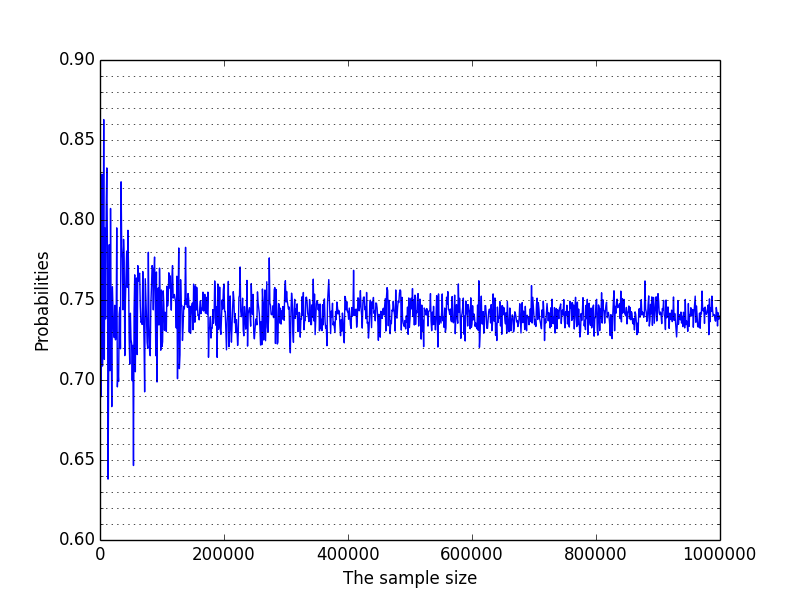
\includegraphics[height=5cm]{32.png}
\subsection *{(d)}
\inputpython {stochastic.py}{1}{51}
\section *{3.3 Node clustering}
\begin{table}[!hbp]
\begin{tabular}{|c|c|c|c|c|c|c|c|}
\hline
$Y_1$&$Y_2$&$Y_3$&$Y$&$P(Y|X=0)$&$P(Y|X=1)$&$P(Z_1=1|Y)$&$P(Z_2=1|Y)$\\
\hline
0&0&0&1&0.09375&0.09375&0.9&0.1\\
\hline
1&0&0&2&0.28125&0.09375&0.8&0.2\\
\hline
0&1&0&3&0.09375&0.03125&0.7&0.3\\
\hline
0&0&1&4&0.03125&0.28125&0.6&0.4\\
\hline
1&1&0&5&0.28125&0.03125&0.5&0.5\\
\hline
1&0&1&6&0.09375&0.28125&0.4&0.6\\
\hline
0&1&1&7&0.03125&0.09375&0.3&0.7\\
\hline
1&1&1&8&0.09375&0.09375&0.2&0.8\\
\hline
\end{tabular}
\end{table}
\section *{3.4 Maximum likelihood estimation}
\subsection *{a}
From the lecture, we know the maximum likelihood solution is:\\
$P_{ML}(X_{i+1} = x_{i+1}| Pa_{i+1} = x_{i}) = P_{ML}(X_{i+1} = x_{i+1}| X_{i} = x_{i}) = \frac{\textrm{count}(X_{i+1}=x_{i+1}, X_i=x_i)}{\textrm{count}(X_i=x_i)} $ \\
And in this question, \\
$\textrm{count}(X_{i+1}=x_{i+1}, X_i=x_i) = \textrm{count}_i(x_i, x_{i+1})$\\
$\textrm{count}(X_i=x_i) = \textrm{count}_i(x_i)$\\
So for the CPTs, \\
$P_{ML}(X_{i+1} = x_{i+1}| X_{i} = x_{i}) = \frac{\textrm{count}_i(x_i, x_{i+1})}{\textrm{count}_i(x_i)}$($x_i$ is the possible value for $X_i$)\\
\subsection *{b}
$P_{ML}(X_{i-1} = x_{i-1}| X_{i} = x_{i}) =  \frac{\textrm{count}(X_{i-1}=x_{i-1}, X_i=x_i)}{\textrm{count}(X_i=x_i)} = \frac{\textrm{count}_{i-1}(x_{i-1}, x_{i})}{\textrm{count}_i(x_i)}$\
\subsection *{c}
From the (a), the joint distribution of $\{X_1, X_2, \cdots, X_T\}$ is:\\
$P(X_1, X_2, \cdots, X_T) = P(X_T|X_{T-1})P(X_{T-1}|X_{T-2})\cdots P(X_3|X_2)P(X_2|X_1)P(X_1)$ (because of the conditional independence)\\
$P(X_1, X_2, \cdots, X_T) = \frac{\textrm{count}_{T-1}(x_{T-1}, x_{T})}{\textrm{count}_{T-1}(x_{T-1})} \frac{\textrm{count}_{T-2}(x_{T-2}, x_{T-1})}{\textrm{count}_{T-2}(x_{T-2})} \cdots \frac{\textrm{count}_2(x_2, x_{3})}{\textrm{count}_{2}(x_{2})} \frac{\textrm{count}_1(x_1, x_{2})}{\textrm{count}_1(x_1)}\frac{\textrm{count}_1(x_1)}{\sum\limits_{x_1}\textrm{count}_1(x_1)} = 
\frac{\textrm{count}_{T-1}(x_{T-1}, x_{T})}{\textrm{count}_{T-1}(x_{T-1})} \frac{\textrm{count}_{T-2}(x_{T-2}, x_{T-1})}{\textrm{count}_{T-2}(x_{T-2})} \cdots \frac{\textrm{count}_2(x_2, x_{3})}{\textrm{count}_{2}(x_{2})} \frac{\textrm{count}_1(x_1, x_{2})}{m}$ (where m denotes the number of examples)\\
From the (b), the joint distribution of $\{X_1, X_2, \cdots, X_T\}$ is:\\
$P(X_1, X_2, \cdots, X_T) = P(X_1|X_2)P(X_2|X_3)\cdots P(X_{T-3}|X_{T-2})P(X_{T-2}|X_{T-1})P(X_T)$ (because of the conditional independence)\\
$P(X_1, X_2, \cdots, X_T) =  \frac{\textrm{count}_{1}(x_{1}, x_{2})}{\textrm{count}_{2}(x_{2})} \frac{\textrm{count}_{2}(x_{2}, x_{3})}{\textrm{count}_{3}(x_{3})} \cdots \frac{\textrm{count}_{T-1}(x_{T-2}, x_{T-1})}{\textrm{count}_{T-1}(x_{T-1})} \frac{\textrm{count}_{T-1}(x_{T-1}, x_{T})}{\textrm{count}_T(x_{T})}\frac{\textrm{count}_T(x_T)}{\sum\limits_{x_1}\textrm{count}_{T}(x_T)} = 
\frac{\textrm{count}_{1}(x_{1}, x_{2})}{\textrm{count}_{2}(x_{2})} \frac{\textrm{count}_{2}(x_{2}, x_{3})}{\textrm{count}_{3}(x_{3})} \cdots \frac{\textrm{count}_{T-1}(x_{T-2}, x_{T-1})}{\textrm{count}_{T-1}(x_{T-1})} \frac{\textrm{count}_{T-1}(x_{T-1}, x_{T})}{m} \\= \frac{\textrm{count}_{T-1}(x_{T-1}, x_{T})}{\textrm{count}_{T-1}(x_{T-1})} \frac{\textrm{count}_{T-2}(x_{T-2}, x_{T-1})}{\textrm{count}_{T-2}(x_{T-2})} \cdots \frac{\textrm{count}_2(x_2, x_{3})}{\textrm{count}_{2}(x_{2})} \frac{\textrm{count}_1(x_1, x_{2})}{m}$ (which is equal to the distribution given by the maximum likelihood CPTs for $G_1$ \\
So the maximum likelihood CPTs for G1 and G2 from this data set give rise to the same joint distribution over the nodes $\{X1, X2, . . . , XT $\}\\
\section *{3.5 Statistical language modeling}
\subsection *{(a)}
The tokens start with the letter 'M' and their numerical unigram probabilities are:\\
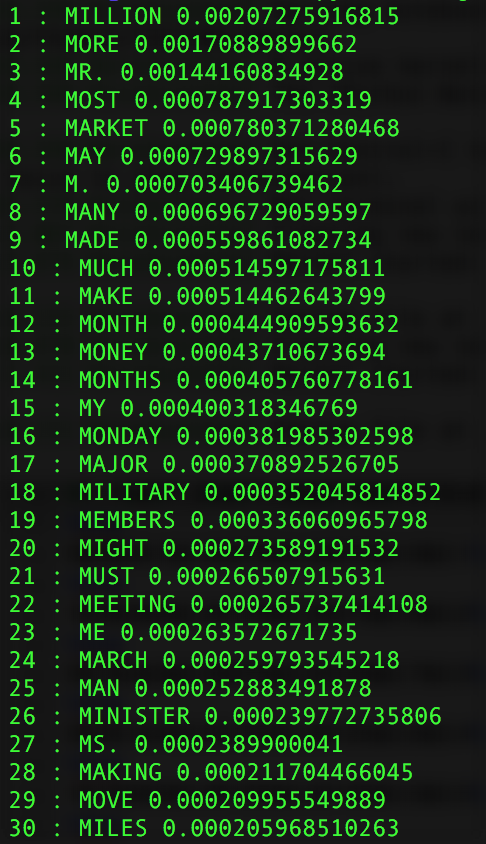
\includegraphics[height=15cm]{35a.png}
\subsection *{(b)}
The ten most likely words to follow the word "THE" and their numerical bigram probabilities are:\\
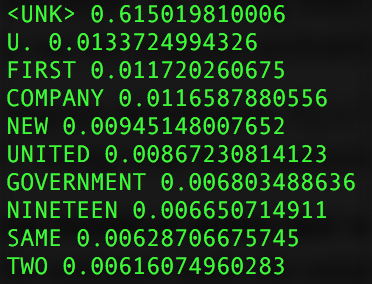
\includegraphics[height=5cm]{35b.png}
\subsection *{(c)}
For this sentence, $\mathcal{L}_u = -64.5094403436$ while $\mathcal{L}_b = -40.9181321338$, so the bigram model yields the highest log-likelihood.\\
\subsection *{(d)}
The pairs (sixteen, officials) and (sold, fire) are not observed in the training corpus, which causes the  likelihood to be 0, namely, the log-likelihood to be $-\infty$.\\
\subsection *{(e)}
The lambda corresponding to the maximum log-likelihood is roughly 0.6491\\
The plot is as follow:\\
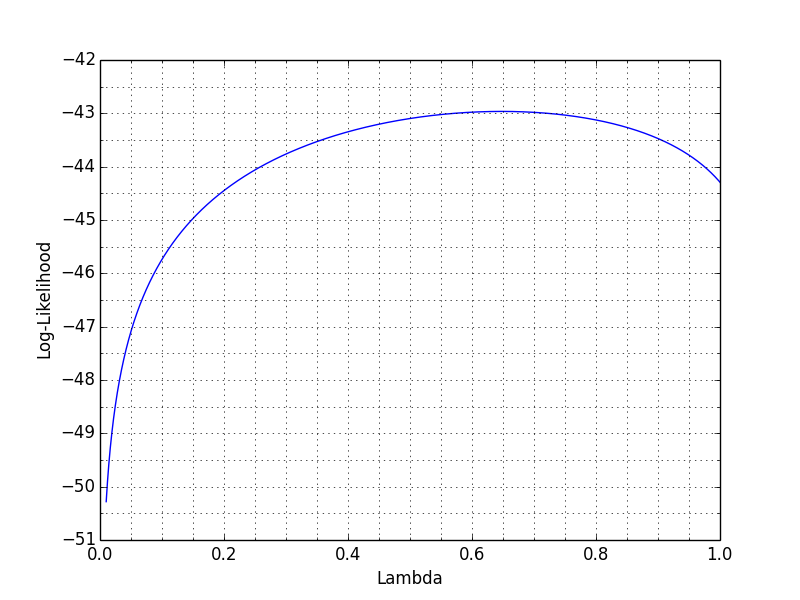
\includegraphics[height=10cm]{35e.png}
\inputpython {lang.py}{1}{122}
\end {document}